% Use only LaTeX2e, calling the article.cls class and 12-point type.

\documentclass[12pt]{article}

% Users of the {thebibliography} environment or BibTeX should use the
% scicite.sty package, downloadable from *Science* at
% www.sciencemag.org/about/authors/prep/TeX_help/ .
% This package should properly format in-text
% reference calls and reference-list numbers.

\usepackage{scicite}

% Use times if you have the font installed; otherwise, comment out the
% following line.

\usepackage{times}

% Package for automaticall generating the table of contents

\usepackage[utf8]{inputenc}

% managing images
\usepackage{graphicx}
\graphicspath{ {images/} }
\usepackage{wrapfig}
\usepackage{amsmath}

\usepackage{setspace}
\onehalfspacing
\setlength{\parskip}{6pt}

\usepackage{physics}

\usepackage[margin=1in]{geometry}

% The preamble here sets up a lot of new/revised commands and
% environments.  It's annoying, but please do *not* try to strip these
% out into a separate .sty file (which could lead to the loss of some
% information when we convert the file to other formats).  Instead, keep
% them in the preamble of your main LaTeX source file.


% The following parameters seem to provide a reasonable page setup.



%The next command sets up an environment for the abstract to your paper.

\newenvironment{sciabstract}{%
\begin{quote} \bf}
{\end{quote}}


% If your reference list includes text notes as well as references,
% include the following line; otherwise, comment it out.

\renewcommand\refname{References and Notes}

\newcounter{lastnote}
\newenvironment{scilastnote}{%
\setcounter{lastnote}{\value{enumiv}}%
\addtocounter{lastnote}{+1}%
\begin{list}%
{\arabic{lastnote}.}
{\setlength{\leftmargin}{.22in}}
{\setlength{\labelsep}{.5em}}}
{\end{list}}


% Include your paper's title here

\title{An Introduction to Quantum Computing} 


% Place the author information here.  Please hand-code the contact
% information and notecalls; do *not* use \footnote commands.  Let the
% author contact information appear immediately below the author names
% as shown.  We would also prefer that you don't change the type-size
% settings shown here.

\author
{Robert Olsthoorn\\
\\
\normalsize{University of Florida}\\
\normalsize{PHY3101: Modern Physics}\\
\normalsize{Fall 2015}\\
}

% Include the date command, but leave its argument blank.

\date{}



%%%%%%%%%%%%%%%%% END OF PREAMBLE %%%%%%%%%%%%%%%%

\begin{document} 



% Double-space the manuscript.

% Make the title.

\begin{figure}
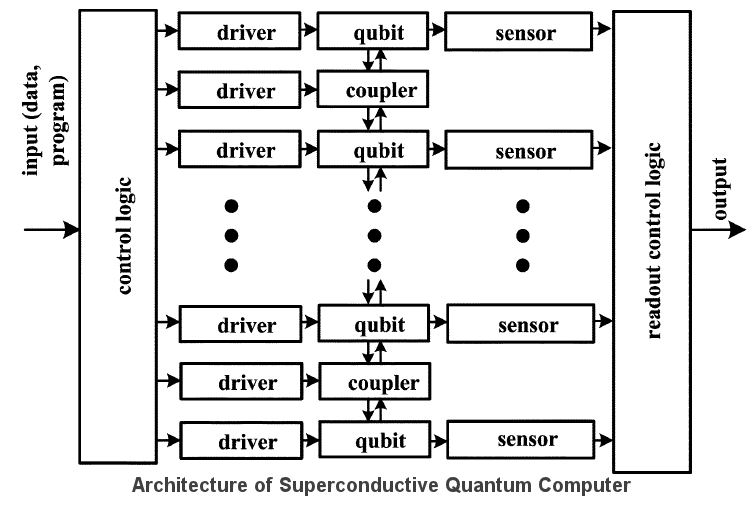
\includegraphics[scale=.5]{superconductive}
\centering
\end{figure}

\maketitle 

% Place your abstract within the special {sciabstract} environment.

\newpage

\begin{sciabstract}
\section*{Abstract}
Quantum computing is a potentially revolutionary principle which will be continued to be researched and studied for the foreseeable future as the importance of efficiency and the limit of binary computing is approached. This paper aims to provide an overview of the field of quantum computing for individuals with a minor understanding of physics, computer science, and mathematics. An introduction to quantum computing will leave the reader with a comfortable overview of the field and insight into which topic in particular they find most interesting.\par
This paper will talk briefly about the recent history of quantum computing as well as a small subset of quantum mechanicss as it relates to quantum computations and the cornerstones which currently make quantum computing possible. It aims to establish the differences between conventional and quantum computing with a goal to speak about how certain algorithms will run more efficiently and what applications in the field this can be used for. Near the end, we will look at the current issues within the field and its future importance.

\end{sciabstract}

\newpage

\tableofcontents

\newpage

\section{History}

Quantum computing is a relatively new field in relation to computer science as a discipline with the informal start originating in the late 1970's and early 1980's as Richard Feynman speculated that quantum mechanics could not be effectively modeled through a classical computer. In accordance with Moore's law, the size of a silicon ship would continue to shrink until the individual elements were no larger than several atoms and would be subject to quantum effects at that scale. Feynman published an abstract model in 1982 in which he analyzed the outcome of using a quantum simulator in order to avoid the exponential slowdown which is common with classical computers.\cite{web}\par
In 1985, David Deutsch published a paper proving that any physical process could be, in theory, effectively rendered on a quantum computer. As a result, a quantum computer, which is able to operate in an exponential time, could provide a wide array of values for heavy data crunching, modelling of complex systems, or in the general solving NP-Complete classical problems in polynomial time.
\footnote{In computational complexity theory, a decision problem is NP-complete when it is both in NP and NP-hard. The set of NP-complete problems is often denoted by NP-C or NPC. The abbreviation NP refers to ``nondeterministic polynomial time''.\\Although any given solution to an NP-complete problem can be verified quickly (in polynomial time), there is no known efficient way to locate a solution in the first place.}
Deutsch proved a basic algorithm which will be worked through later in the paper. \par
Until 1994, the quantum computing field remained relatively unchanged until Shor was able to prove and set a method for a common NP-Hard factorization problem which could call on the benefits allowed through quantum computers, which would run in a time much shorter than what will be ever possible on classical computers.\cite{web} As a field, this momentus finding was able to push the field of research for quantum computing out of the view of the select who were performing research on the project to the public eye. Shor's algorithm will be explored later in the paper as well.\par

\section{Quantum Concepts and Theories}

As a quick note, the material that will only be covered consists of a very small section of quantum mechanics encompassing finite dimenstional quantum mechanic where the vector spaces which represent the states of the dimension are finite in size.\par

\subsection{Double Slit Experiment}
Young's double slit experiment is one of the most foundational experiments related to the field of quantum mechanics and demonstrates the wave-particle duality of photons when conducted. Before approaching the quantum model, it is interesting to explore a classical model and the probabilities associated with it before moving on.\par
\begin{wrapfigure}{l}{0.5\textwidth}
  \centering
  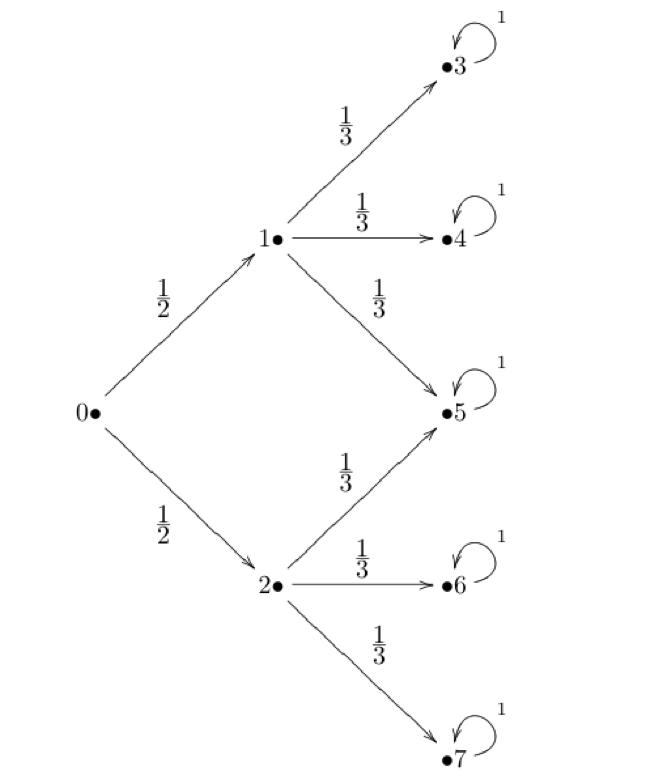
\includegraphics[width=0.5\textwidth]{classicslit}
  \caption{Corresponding graph to scenario}
\end{wrapfigure}
Pretend for a moment, that there is an experiment where there is a sharpshooter who is guaranteed to always shoot through one or the other open windows, with equal probability. Once the bullet passes through the window, it has an equal probability of hitting three targets. There is one target which is shared between both open windows.\par
The probability matrix associated with this scene is shown. 
\begin{figure}
  \centering
  \caption{Matrix representing the progression after one time click}
  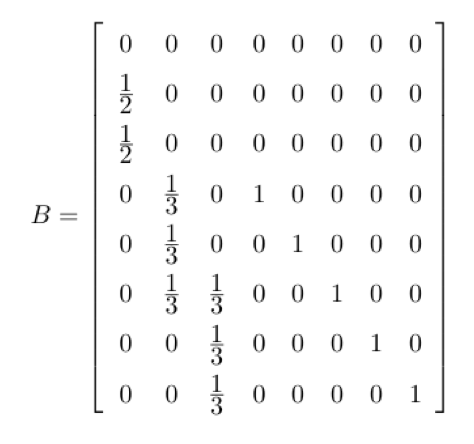
\includegraphics{classicB}
\end{figure}
\par
By representing the data points as a matrix, it is possible to identify the probability where the bullet might be found on the next time click by simply using matrix multiplication.\cite{intro}. The matrix shown above, \textit{B}, represents the state of the system after one time click. By multiplying the matrix by itself you are able to represent the state after two time clicks. 
\begin{figure}
  \centering
  \caption{Matrix representing the progression of two time clicks}
  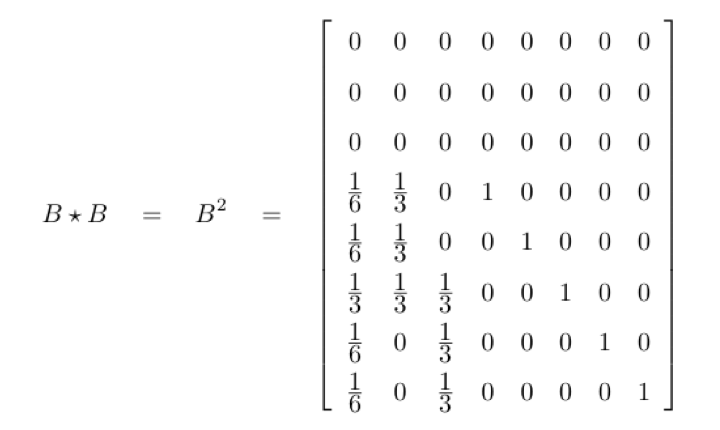
\includegraphics[width=0.5\textwidth]{classicB2}
\end{figure}\par
The takeaway from this example is to show that after two time clicks the bullets will be in the state \[B^2X = [0,0,0,\frac{1}{6},\frac{1}{6},\frac{1}{3},\frac{1}{6},\frac{1}{6}]^T\]
Which means that \(B^2[5,0]\) is equivalent to \(\frac{1}{3}\). Which is the two states \(\frac{1}{6}+\frac{1}{6}\).\par

\begin{wrapfigure}{l}{0.5\textwidth}
    \centering
    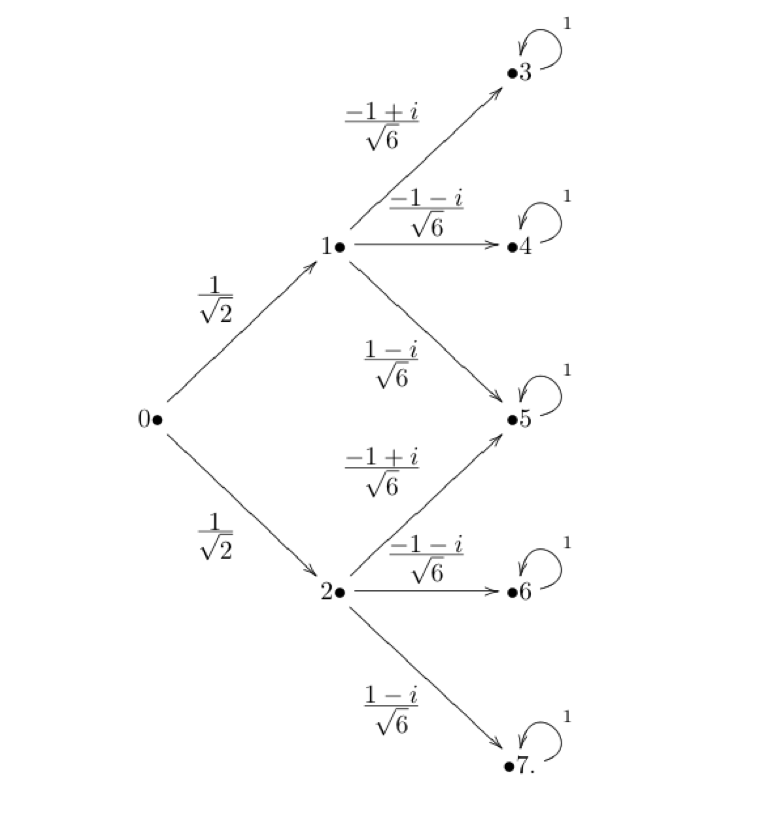
\includegraphics[width=0.5\textwidth]{quantumslit}
    \caption{Corresponding quantum modulus graph to scenario}
\end{wrapfigure}
Pretend for a moment that the shooter has now been changed to a flashlight which can spread light into both of the windows with a similar setting. Once the light has passed through the windows, it again travels randomly to one of the three respective target locations. Represented in this graph is the modulus, where the modulus squared represents the probabibility of the specific event taking place. $\frac{1}{\sqrt{2}}^2$ is $\frac{1}{2}$ and more importantly $\left|\frac{\pm 1 \pm i }{\sqrt{6}}\right|^2 = \frac{1}{3}$  \footnote{The complex number weights represented here are not to represent the actual quantum probability weights as this would require acquiring the distance of the slit spacing, the width of the individual slits. Rather the numbers given are to represent the point of quantum interference which will be highlighted later on}
\begin{figure}
	\centering
	\caption{Matrix representing the state after one time click}
	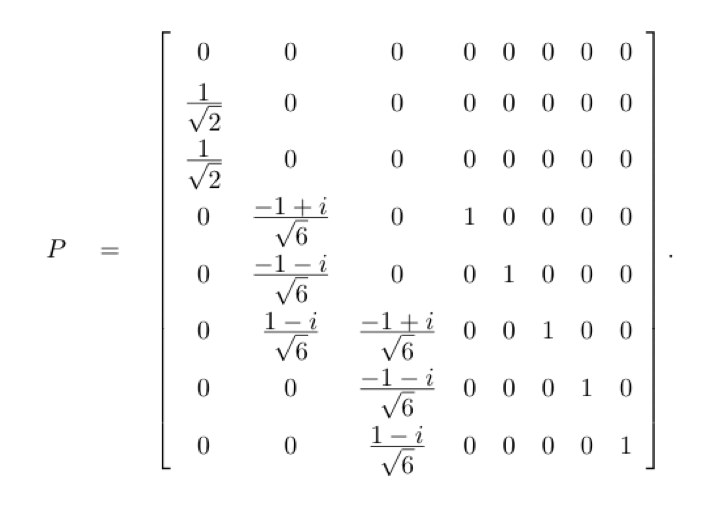
\includegraphics[width=.5\textwidth]{quantumP}
\end{figure}
\begin{figure}
	\centering
	\caption{Matrix representing the state after two time clicks}
	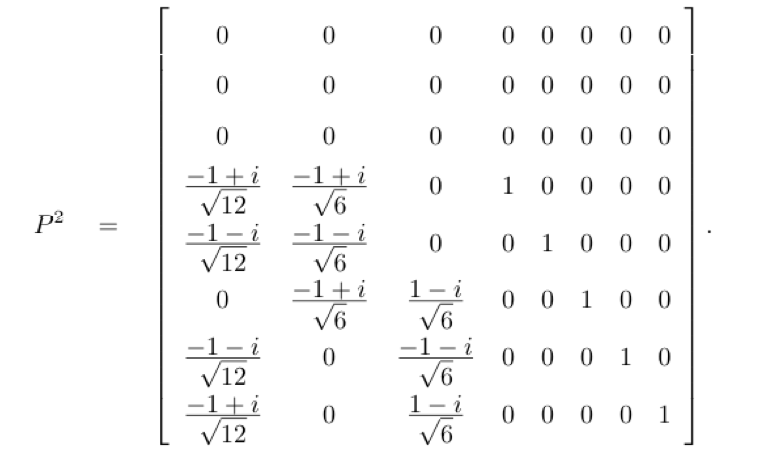
\includegraphics[width=.5\textwidth]{quantumP2}
\end{figure}
The above matrices represented the state of the experiment using the moduli of the components. In order to interpret this information in reference to the classical scenario it is helpful to consider the probability of the individual locations. This can be shown by squaring the individual components of the $P^2$ matrix.
\begin{figure}
	\centering
	\caption{Probability matrix of the modulus squared after two time clicks}
	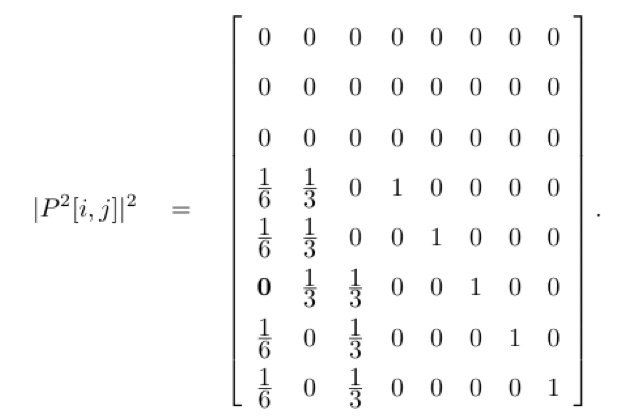
\includegraphics[width=.5\textwidth]{quantumProbability}
\end{figure}
\par
For the most part, the probability matrix for $P^2$ is the same as the probability matrix for $B^2$; however, there is one important distinction to be made. Which is that while $B^2[5,0] = \frac{1}{3}$ in the quantum simulation $P^2[5,0] = 0$. On a mathematical basis, this is trivially written as 
$$\frac{1}{\sqrt{2}}\bigg(\frac{-1+i}{\sqrt{6}}\bigg) + \frac{1}{\sqrt{2}}\bigg(\frac{1-i}{\sqrt{6}}\bigg) = \frac{-1+i}{\sqrt{12}} + \frac{1-i}{\sqrt{12}} = 0$$
This may seem troubling at first, but it must be remembered that photons are subject to particle interference and thus, on the shared target of the windows, the probability drops to 0. Furthermore, one may try to argue that if the experiment was carried out using only one photon, then the probability would again return to $\frac{1}{3}$, but this assumption would also be incorrect. A single photon is said to have a superposition in being in every possible position simultaneously. This is not mimicked in the classical world; however, due to the photon residing in every position at once it is prone to interference when the shared target is reached. As with most quantum phenomena, the particle is only determined to be in a certain state with a certain probability when a measurement is taken. In quantum mechanics, a measurement causes the superposition state to collapse to a certain pure state.\cite{intro}\par
This phenomena is central to the success of quantum computing, as it allows for an exponential number of comutations or simulations to be run in parallel thus becoming exponentially more efficient.

\subsection{Unitary Transformations}
The complex numbers which represent the quantum position are commonly known as the amplitudes of the wave function. A core theory in regards to quantum systems is the idea of a unitary transformation. Provided that the entire amplitude function $\Psi$ can be identified through a vector, a unitary transforamtion is a multiplication of those vectors by a transformation matrix whose inverse equals its conjugate transpose. \cite{cis4930}
The inherent properties of unitary transformations indicate that the total probability of the set always remains the same where the sum of the squares of the amplitudes is equivalent to 1 and that all changes are preserve the information across all states. Once a quantum state is observed in an isolated system, the quantum state is determined for all past and future times.\par
Furthermore, unitary transformations are fully reversible. This property can be shown to be true because $\ket{\psi} \mapsto U\ket{psi}$ preserves the normal standardization across states it can then be set that $1 = \bra{\psi}\ket{\psi} = \bra{\psi}U^ \dagger U\ket{\psi} $ for all unit vectors $\ket{\psi}$. By linearity it follows that $U^\dagger U = I$ which indicates invertibility. 
\footnote{The format used is known as bracket notation and will be understood in the following subsection. Where the $\bra{x}$ represents the ``bra'' section and the $\ket{x}$ represents the ``ket'' section and the entire representation can be shown by $\bra{x}\ket{x}$}

\subsection{Bracket Notation}
An $n$ dimensional quantum system indicates that a particle can be in one of $n$ states or positions. The quantum system could also represent the energy level of the photon polarization direction; however, for the purpose of defining the bracket notation consider just the position of the particle.\footnote{This section focuses on the ``ket'' of the bracket notation. The matching ``bra'' $\bra{x}$ denotes the conjugate transpose of $\ket{x}$. This choice is arbitrary, but is the convention which is widely used when talking about quantum computing \cite{non}}\par
The state $$\ket{\psi} = [0,1,0,0,...,0]^T$$ is to represent that the particle is found at position 1. Similarly the state $$\ket{\psi'} = [0,...,1,...,0]^T$$ is said to be found at the position $j$ where the particle can be found. These states, where the particle can be certainly found are known as pure states. A superposition of the general form $$\ket{\phi} = [c_0, c_1,...,c_{j},...,c_{n-1}]^T$$ can be added to another superposition state simply by adding elements individually. Adding the inital to $$\ket{\phi'} = [c_0', c_1',...,c_{j}',...,c'_{n-1}]^T$$ yields
$$\ket{\phi} + \ket{\phi'} = [c_0+c_0', c_1+c_1', ..., c_{j}+c'_{j},..., c_{n-1} + c'_{n-1}]^T$$ This process of adding the complex vector spaces are valid and yied accurate results.\par
The only component which matters is not the length $\ket{\phi}$, but the direction of the component. Working with these vectors, it makes more sense to work with a normalized version of the vector $$\frac{\ket{\phi}}{\left|\ket{\phi}\right|}$$\par

While this works for adding the superposition states together in order to combine quantum systems it becomes necessary to calculate the tensor product \footnote{SOME INFORMATION ON THE TENSOR PRODUCT PLACED IN HERE}. If we take $\ket{\phi}$ to be the first quantum system and take $\ket{\phi'}$ to be the second quantum system we represent the combined system as $$\ket{\phi}\otimes\ket{\phi'} = \ket{\phi, \phi'} = \ket{\phi \phi'}$$

\subsection{Observations}
As mentioned before, when a quantum superpositiion state it condenses to a single pure state in order for the experiment to show the particle at a single position. In an attempt to predict which state the particle will condense to we look at the sum of the squares of the modulus\cite{intro} 
$$S = \left|c_0\right|^2 + \left|c_1\right|^2 + \left|c_{j}\right|^2 +\left|c_{n-1}\right|^2$$ 
Therefore there is a $\left|c_0\right|^2\!/S$ chance of the superposition collapsing to the $0th$ pure state and a $\left|c_1\right|^2\!/S$ chance of collapsing to the $1st$ pure state as the way that the quantum state collapses is random, but can be represented as a hermitian.
\footnote{an $ n\times n $ matrix is considered hermition if $A = A^\dagger $. In other words, only if $ A^T = \overline{A} $}
\par
\textbf{Eigenvalue} is a real number which can be found in a hermitian matrix if for a matrix $A$ in $M^{n\times ns}$, there is a number $m$ in $M$ and a vector $\ket{\phi}$ in $M^n$ such that $A\ket{\phi} = m\ket{\phi}$. $m$ in this case is an Eigenvalue, where $\ket{\phi}$ is known as a \textbf{Eigenvector} of $A$ associated with $m$.\par
All eigenvalues in a hermitian matrix are all real numbers. Furthermore, distinct eigenvectors which have distinct eigenvalues of a hermitian matrix are orthogonal. It follows that the set of eigenvectors form a basis for the entire complex vector space which represents the quantum of interest. \cite{intro}. Taking $A\ket{\phi} = m\ket{\phi}$, it becomes obvious that, as stated before, the only part of the state that matters is the direction rather than the length. This means that $m\ket{\phi} = \ket{\phi}$ A critical assumption which can be made following this statement is that if the current state of the quantum system is based on the eigenvector basis, than the system will not change.
\section{Qubit}
Fundamentally, a bit is the state of any system. A classical bit represents one of two distinct positions for a scenario as in a 1 or 0, on or off, true or false. In classical computers all data is stored, shuttled, and interpreted through 1's or 0's. Due to the binary state of data, this limits the number of computations that can be done at any single time on a classical machine.\par
Quantum bits (qubits), rather, is a unit vector in a two dimensional complex vector space. When observed a quantum bit will settle into either a $\ket{0}$ or $\ket{1}$ binary state. The implementation of a qubit could correspond to the polarization of the photon or the spin-up or spin-down components of an electron.\cite{non} A quantum bit can be represented as a superposition of $\ket{0}$ or $\ket{1}$ such that $a\ket{0}+b\ket{1}$ where $a$ and $b$ are complex numbers such that $\left| a\right |^2+\left| b\right| ^2 = 1$.\par
An important consideration is that the state can only be measured once. Though it may seem possible to clone a qubit so that it may be measured in two possible ways, this is impossible. Because quantum states are subject only to unitary transformations, cloning is not allowed. The proof, established in 1982 by Wooters and Zurek, is an example of the linearity of unitary transformations.\cite{non}\par
Assume that $U$ is a unitary transformation which is possible to clone so that in all quantum states $\ket{a}, U(\ket{a0}) = \ket{aa}$. Let $\ket{a}$ and $\ket{b}$ be orthogonal quantum states. And $U(\ket{a0}) = \ket{aa}$ and $U(\ket{b0}) = \ket{bb}$. Consider the case $\ket{c} = (1/\sqrt{2})(\ket{a} + \ket{b})$.
\begin{align*}
U(\ket{c0} &= \frac{1}{\sqrt{2}}(U(\ket{a0})+U(\ket{b0}))\\
&= \frac{1}{\sqrt{2}}(\ket{aa}+\ket{bb})
\end{align*}
But since U was defined as a cloning transformation
\begin{align*}
U(\ket{c0}) &= \ket{cc}\\
&= (\frac{1}{\sqrt{2}}(\ket{aa}+\ket{bb}))^2\\
&= \frac{1}{2}(\ket{aa}+\ket{ab}+\ket{ba}+\ket{bb})
\end{align*}
which is not equal to $1/sqrt{2}(\ket{aa}+\ket{bb})$. This proves that there is no unitary operation to clone unknown quantum states. This \textit{no cloning} principle is only valid for unknown quantum states, as it is in fact possible to clone known quantum states. Though it is possible to obtain particles in an entangled state from an unknown state.

\subsection{Notation}
\subsection{Implementation}
\section{Applications}
\subsection{Implementation}
\section{Algorithms}
\subsection{Shor's Algorithm}
\subsection{Grover's Algorithm}
\subsection{Deutsch Algorithm}
\section{Error Correction and Measurement}
\section{Future of Quantum Computing}


\begin{figure}
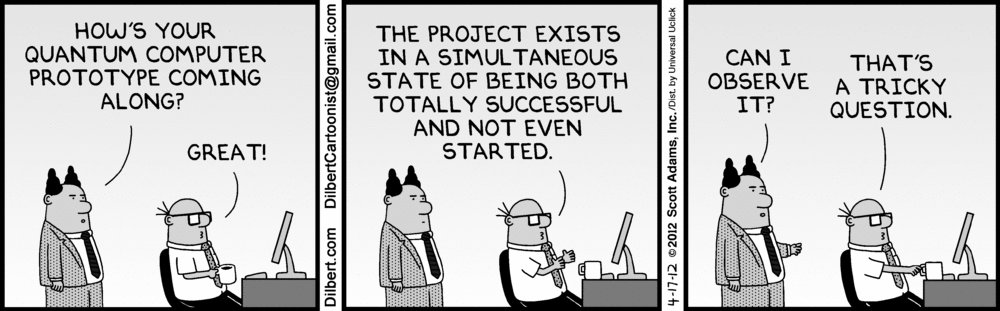
\includegraphics[scale=.5]{dilbert}
\centering
\end{figure}

% Your references go at the end of the main text, and before the
% figures.  For this document we've used BibTeX, the .bib file
% scibib.bib, and the .bst file Science.bst.  The package scicite.sty
% was included to format the reference numbers according to *Science*
% style.


\bibliography{scibib}

\bibliographystyle{Science}

\newpage

\begin{thebibliography}{1}
\bibitem{pro} 
Preskill, John. ``Quantum Computing: Pro and Con.'' Diss. California Instute of Technology, 1996. Print. Covers the applications in which it will be used as well as the technical difficulties that are encountered with creating a quantum computer. Also encompasses the future of quantum computing
\bibitem{non}
Rieffel, Eleanor, and Wolfgang Polak. ``An Introduction to Quantum Computing for Non-Physicists.'' Diss. FX Palo Alto Laboratory, 2000. Print. Covers some algorithm efficiencies for conventional vs quantum computing and also covers basic applications of quantum computing in the field including cryptography.
\bibitem{web}
West, Jacob. ``The Quantum Computer.'' An Introduction to Quantum Computing. Rice University, 28 Apr. 2000. Web. 25 Oct. 2015. Provides a general purpose overview of the field of quantum computing. Includes a brief history of the field as well as current obstacles and research being done in the field.
\bibitem{intro}
Yanofsky, Noson S. ``An Introduction to Quantum Computing.'' Diss. Department of Computer and Information Science, Brooklyn College, CUNY, 2007. Print. Presents an introduction to the mathematics behind quantum computing as well as an overview of the architecture necessary for quantum computing. This paper also presents Deutsch's Algorithm which will be spoken about and overviewed.
\bibitem{cis4930}
CIS4930 Textbooks
\end{thebibliography}

\clearpage

\end{document}




















